%-------------------------
% Rover Resume - Office Template
% Link: https://github.com/subidit/rover-resume
%------------------------

\documentclass{article}

\usepackage{lmodern}
\usepackage[T1]{fontenc}

\usepackage[sfdefault,light]{FiraSans}
\usepackage{geometry}
\geometry{a4paper,margin=0.8in,top=0.5in,bottom=0.5in}
\pagestyle{empty}
\setcounter{secnumdepth}{0}
\usepackage{microtype}
\usepackage{graphicx}
\usepackage{fontawesome5}
\usepackage{enumitem}
\setlist[itemize]{leftmargin=*,label=\faCaretRight,itemsep=0pt}
\usepackage{xcolor}
\definecolor{background}{HTML}{0D47A1}
\usepackage[explicit]{titlesec}
\titleformat{\section}{\large\bfseries\color{white}}{}{}{\colorbox{background}{#1}}
\titleformat{\subsubsection}{\large\itshape}{}{}{#1}
\titlespacing{\subsection}{0pt}{*3}{*0.5}
\titlespacing{\subsubsection}{0pt}{*0}{*0.5}

\newcommand{\rside}[1]{\hfill \normalfont\scshape\MakeLowercase{#1}}

\usepackage[bookmarks=false,hidelinks]{hyperref}

\begin{document}

\begin{center}
  \begin{minipage}{0.45\textwidth}
    {\Huge\bfseries Pedro Paulo \\ Almeida Rodrigues} \\[0.5ex] 
  \end{minipage}\hfill
  \begin{minipage}{0.35\textwidth}
    \faPhone\ (96) 99184-9667 \\
    \href{mailto:apedropaulo20@gmail.com}{\faEnvelope\ apedropaulo20@gmail.com} \\
    \href{https://www.linkedin.com/in/pedro-paulo-almeida-rodrigues-a788541a1}{\faLinkedin\ Pedro Paulo Almeida Rodrigues} \\
    \href{https://github.com/PedroPaulo-98}{\faGithub\ PedroPaulo-98}
  \end{minipage}
  \begin{minipage}{0.15\textwidth}
    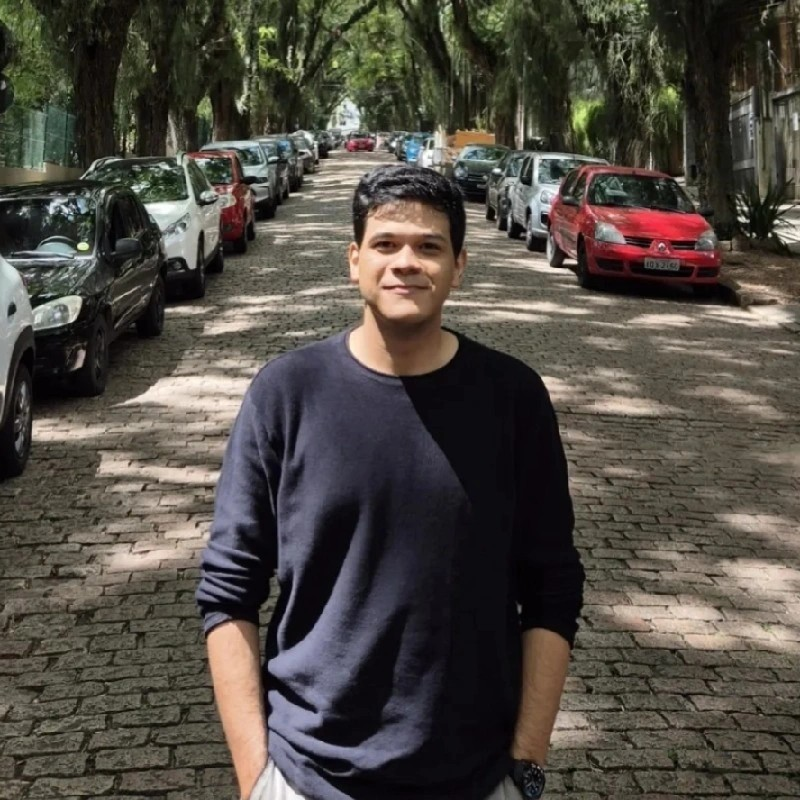
\includegraphics[width=\linewidth]{pedro.jpg}
  \end{minipage}
\end{center}

\section{\faUser\enspace Sobre o Pedro}
%========
\begin{description}
  \item \ \ \ \ \ \  Sou um profissional apaixonado por tecnologia e educação. Atuo como Analista de Sistemas no PRODAP, onde desenvolvo e presto suporte a sistemas governamentais do estado do Amapá além de desenvolver sistemas para empresas. Tenho experiência no desenvolvimento de software utilizando frameworks como Django, Laravel, fastAPI e outros. Meu objetivo é contribuir para a inovação e melhoria da qualidade de vida por meio da tecnologia e da educação. \\ Sou resiliente buscando aprender e me adaptar rapidamente, busco sempre ter um bom relacionamento em grupo, tendo sentido de responsabilidade e capacidade em lidar com situações de pressão
\end{description}

\section{\faCogs\enspace Habilidades}
%========
\begin{description}
  \item[Traços] Trabalhador, Resiliente, Paciente, Dedicado
  \item[Experiências] PHP, Laravel, Python, FastAPI, Django, Flutter, Java, Quarkus, SQL, GIT, Docker, BI, Dashboards, Mikrotik, entre outras tecnologias
\end{description}

\section{\faChartPie\enspace Experiencias}
%================

\subsection{TGR Studio (PJ)\rside{Maio 2025 - Até o momento}}
\subsubsection{Desenvolvedor Full Stack PJ \rside{Novo Hamburgo, RS}}
\begin{itemize}
  \item Desenvolvimento de sistemas (Laravel)
  \item Plataformas de E-commerce
\end{itemize}

\subsection{PRODAP - Centro de Gestão da Tecnologia da Informação (Contrato) \rside{Abril 2024 - Até o momento}}
\subsubsection{Analista de Sistemas (Desenvolvedor) \rside{Macapá, AP}}
\begin{itemize}
  \item Desenvolvimento de sistemas e APIs (Laravel, Django e FastAPI)
  \item Atualizações e melhorias de sistemas legados (PHP 5 e 7, Laravel 5 e 7)
  \item Análise de dados com dashboards (Lookerstudio, Python, Django e Plotly)
\end{itemize}

\subsection{PRODAP - Centro de Gestão da Tecnologia da Informação (Contrato) \rside{Junho 2023 - Abril 2024}}
\subsubsection{ Analista de Dados  \rside{Macapá, AP}}
\begin{itemize}
  \item Coleta de dados e desenvolvimento de dashboards do estado do Amapá
  \item Criação do vacinômetro AP (http://srag.painel.prodap.ap.gov.br/vacinometro.html)
  \item Sistema de compromissos governamentais
\end{itemize}

\subsection{Faculdade de Tecnologia do Amapá Meta (CLT)  \rside{Janeiro - Junho 2024}}
\subsubsection{ Professor Universitário  \rside{Macapá, AP}}
\begin{itemize}
  \item Matéria de Arquitetura e organização de computadores
  \item Matéria de Redes de computadores
  \item Matéria de Introdução à Engenharia da Computação
\end{itemize}


\subsection{SESA - Secretaria Estadual de Saúde do Amapá (Contrato) \rside{Março 2023 - Abril 2024}}
\subsubsection{ Desenvolvedor e Analista de Gestão de Projetos  \rside{Macapá, AP}}
\begin{itemize}
  \item Desenvolvimento de sistemas na área da saúde (PHP com o framework Laravel)
  \item Acompanhamento da infraestrutura de redes nos hospitais do estado do Amapá
  \item Criação do sistema SSD-AP (Sistema de Saúde Digital do Amapá).
\end{itemize}

\subsection{IFAP – Instituto Federal de Educação, Ciência e Tecnologia do Amapá (Contrato) \rside{Abril - Junho 2023}}
\subsubsection{ Professor de Informática  \rside{Mazagão, AP}}
\begin{itemize}
  \item Professor de informática básica no projeto Mais Cultura no Meio do Mundo
\end{itemize}

\subsection{Estágios}
\subsubsection{Corumba Outsourcing - Suporte \rside{2019}}
\begin{itemize}
  \item Suporte em empresas
  \item Manutenção de computadores
  \item Criação de relatórios para melhorias
\end{itemize}
\subsubsection{PRODAP - Governança de TI \rside{Novembro 2020 - Novembro 2022}}
\begin{itemize}
  \item Coleta e organização de dados da autarquia para criação de dashboards e relatórios
  \item Criação de políticas de uso de sistemas
  \item Acompanhamento na aplicação de metodologias ágeis
\end{itemize}

\section{\faGraduationCap\enspace Formação}
%==========
\subsection{Faculdade de Tecnologia do Amapá Meta  \rside{Janeiro 2017 - Junho 2022}}
\subsubsection{Engenharia de Computação \rside{Macapá, AP}}
\begin{itemize}
  \item \textit{SINALIZADOR AUTOMOTIVO PARA PESSOAS COM DEFICIÊNCIA AUDITIVA}
  \item \textit{UTILIZAÇÃO DE UM MICROCOMPUTADOR COMO SERVIDOR PROXY PARA MICRO E PEQUENAS EMPRESAS}
  \item \textit{SISTEMA DE ACOMPANHAMENTO E GERENCIAMENTO DE EPI ATRAVÉS DE RFID}
\end{itemize}
%==========
\subsection{Instituto Federal de Educação, Ciência e Tecnologia do Amapá (IFAP) \rside{Julho 2022 - Dezembro 2023}}
\subsubsection{Pós-Graduação em Informática na Educação \rside{Macapá, AP}}
\begin{itemize}
  \item \textit{UTILIZAÇÃO DO APLICATIVO EDUC-BIO: como estratégia de ensino de biologia para alunos do 3º ano das escolas públicas de Macapá}
\end{itemize}
%==========
\subsection{Pontifícia Universidade Católica do Rio Grande do Sul (PUCRS) \rside{Setembro 2022 - Dezembro 2023}}
\subsubsection{Pós-Graduação em Segurança Digital, Governança e Gestão de Dados \rside{Porto Alegre, RS}}
\begin{itemize}
  \item \textit{SISTEMA DE ACOMPANHAMENTO E GESTÃO DE PROMESSAS POLÍTICAS ATRAVÉS DE UM PAINEL DASHBOARD}
\end{itemize}





\section{\faFlask\enspace Projetos}
%==========

\subsection{Inscrição Amapá Jovem (2024 e 2025)}
\begin{itemize}
  \item Atualização de sistema de inscrição do projeto Amapá Jovem
\end{itemize}

\subsection{Vacinometro}
\begin{itemize}
  \item Sistema de casos e vacinas no estado do Amapá (http://srag.painel.prodap.ap.gov.br/vacinometro.html)
\end{itemize}

\subsection{API Transparência}
\begin{itemize}
  \item API dos dados dos Benefícios Sociais, Servidores e diárias civil e militar
  \item http://api.transparencia.ap.gov.br/docs
\end{itemize}

\subsection{Sistema de RH}
\begin{itemize}
  \item Sistema interno de Recursos Humanos
\end{itemize}

\subsection{Sistema de Saude Digital do Amapá}
\begin{itemize}
  \item Sistema de porta de entrada nos hospitais do estado do Amapá
\end{itemize}

\subsection{Desenvolvimento de sistemas}
\begin{itemize}
  \item Sistemas desenvolvidos em PHP, Laravel, Django, FastAPI e outros 
\end{itemize}

\subsection{Atualizações de sistemas legados}
\begin{itemize}
  \item Sistemas PHP 5 e 7, com Laravel 5 até o 10
\end{itemize}




\href{https://github.com/PedroPaulo-98/Curriculo}{\faGithub\ Currículo no GitHub}

\end{document}